\chapter{Les cycles thermodynamiques}
\section{Introduction}
Un \textbf{cycle} est un ensemble de transformation après lesquelles 
le fluide moteur retourne à son état initial. Un cycle est dit 
\textbf{idéal} lorsqu'il approxime un processus réel. Il s'agit d'une 
approche pratique simplifiée mais non exacte. Dans la réalité, il y a 
toujours des pertes de charges (cf. \textit{PDT}),\dots

	\subsection{Travail réversible}
	Le travail des cycles moteurs est différent si le système est 
	ouvert ou fermé :
	\begin{itemize}
	\item[$\bullet$] Systèmes fermés 
	\begin{equation}
	dw_{rev} = -p.dv
	\end{equation}
	\item[$\bullet$] Systèmes ouverts
	\begin{equation}
	dw_{rev} = v.dp
	\end{equation}
	\end{itemize}
	Il existe toute une série d'expression du travail associés à différents 
	systèmes en fonction des propriétés, liste non reprise ici.
	
	\subsection{Diagramme entropique}
	Il s'agit d'un diagramme $(T,s)$, utilisé pour les échanges de chaleurs 
	car l'aire sous une transformation réversible est la quantité de chaleur 
	échangée 
	\begin{equation}
	\delta q_{rev} = T.ds
	\end{equation}
	L'entropie d'un gaz parfait s'écrit 
	\begin{equation}
	ds = c_p\dfrac{dT}{T}-R\dfrac{dp}{p} = c_v\dfrac{dT}{T}+R\dfrac{dv}{v}
	\end{equation}
	Dans un tel diagramme, les transformations adiabatiques seront représenté 
	par une ligne verticale et les $p,v=\ cste$ par une fonction exponentielle :
	\begin{equation}
	\begin{array}{llll}
	p =\ cste &; ds = c_p\frac{dT}{T},& s = c_p\ln T + B, & T = ke^{\frac{s}{c_p}}\\
	v =\ cste &; ds = c_v\frac{dT}{T},& s = c_v\ln T + B, & T = ke^{\frac{s}{c_v}}	
	\end{array}
	\end{equation}
	\begin{center}
	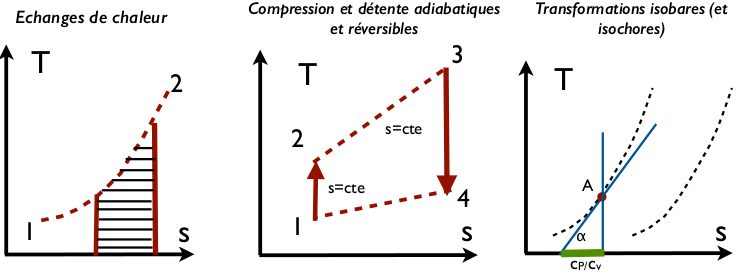
\includegraphics[scale=0.45]{ch9/image1.png}
	\captionof{figure}{NB : $T/C_p = dT/ds = \tan\alpha$}
	\end{center}	
	Dans un diagramme entropique, les isobares et isochores se déduisent par simple
	translations.
	
	\subsection{Diagramme du travail}
	Il s'agit du classique, le diagramme $(p,v)$, très pratique pour les échanges de 
	travail car l'aire située sous une transformation vaut le travail échangé. 
	\begin{equation}
	pv^n=\ cste,\qquad pv = RT\qquad \rightarrow \left\{\begin{array}{ll}
	Tp^{\frac{1-n}{n}}=\ cste\\
	Tv^{n-1}=\ cste	
	\end{array}\right.
	\end{equation}		
	Les transformations polytropiques se représentent ainsi comme des hyperboles 
	et les autres ($pv,=\ cste$) par des lignes droites.
	\begin{center}
	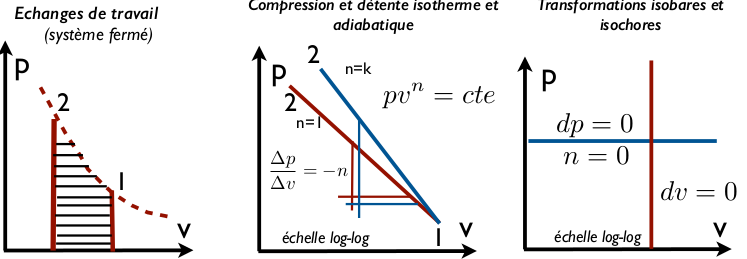
\includegraphics[scale=0.45]{ch9/image2.png}
	\captionof{figure}{Diagrammes $(p,v)$}
	\end{center}	
	
	
	
\section{Cycles à vapeur}
	\subsection{Le cycle de Rankine}		
	Il s'agit du cycle idéal des centrales thermiques à vapeur d'eau. L'idée est 
	qu'une pompe comprime de l'eau (le travail de compression doit être minimal 
	par rapport à celui de la turbine). Une fois comprimé à l'état de liquide 
	saturé, on le chauffe jusqu'à l'état de vapeur saturé pour ensuite le faire 
	détendre dans la turbine. Notre source "froide" est donnée par la condenseur.\\
	Ces quatre étapes sont les suivantes :
	\begin{description}
	\item[1-2] compression adiabatique et réversible dans la pompe (à partir de 
	l'état liquide saturé)
	\item[2-3] échange de chaleur isobare jusqu'à l'état de vapeur saturée
	\item[3-4] détente adiabatique réversible dans la turbine
	\item[4-1] échange de chaleur isobare dans le condenseur
	\end{description}
	\begin{center}
	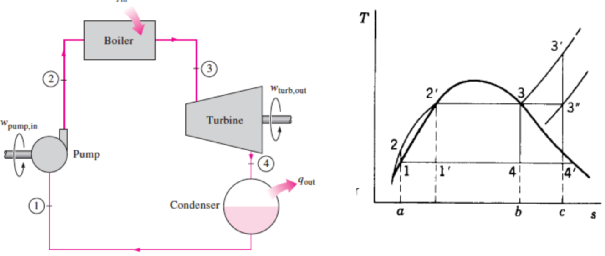
\includegraphics[scale=0.5]{ch9/image3.png}
	\captionof{figure}{Cycle de Rankine}
	\end{center}

	\danger Si on passe dans un surchauffeur, il s'agit du cycle de  Hirn et non 
	plus de Rankine ! Sur le schéma ci-dessus, 3-4 correspond au cycle de Rankine 
	et 3'-4' au cycle de Hirn.
	
		\subsubsection{Travail}
		\begin{wrapfigure}[8]{l}{4cm}
		\vspace{-5mm}
		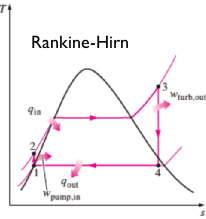
\includegraphics[scale=0.45]{ch9/image4.png}
		\captionof{figure}{ }
		\end{wrapfigure}
		Plus la différence de volume massique entre les phases de détente et de 
		compression est grande, plus le travail effectué sera grand :
		\begin{equation}
		w_{net} = w_{turbine}^* - w_{pompe}
		\end{equation}
		Pour maximiser cette différence, on effectue un changement de phase 
		\begin{equation}
		\begin{array}{ll}
		w_{pompe} &= v_L \int_{p_1}^{p_2} dp = v_L(p_2-p_1)\\
		w_{turbune} &= \int_{p_4}^{p_3} v_Vdp
		\end{array}
		\end{equation}
		Dans ces conditions, le travail de la pompe sera 1k plus petit que celui 
		de la turbine : on le néglige
		\begin{equation}
		v_L \ll v_V \rightarrow w_{pompe} \ll |w_{turbine}|
		\end{equation}
		Pour effectuer le changement de phase, on surchauffe la vapeur avant de 
		la détendre : c'est le \textbf{cycle de Hirn}
		
		\subsubsection{Analyse énergétique}
		\begin{wrapfigure}[8]{r}{4cm}
		\vspace{-5mm}
		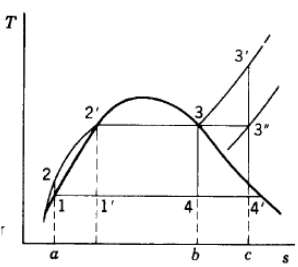
\includegraphics[scale=0.45]{ch9/image5.png}
		\captionof{figure}{ }
		\end{wrapfigure}
		On considère un système \textbf{ouvert} ($q+w = h_2-h_1$), stationnaire, 
		une entrée/sortie et pas de variation de $T$ et $V$. Faisons le bilan :
		\begin{description}
		\item[Pompe ($q=0$)] $w_{pompe} = h_2-h_1 = v(p_2-p_1)=1/\rho(p_2-p_1)$
		\item[Chaudière ($w=0$)] $q_{in} = h_3-h_2$
		\item[Turbine ($q=0)$] $w_{turbine}^* = h_3-h_4$
		\item[Condenseur $(w=0)$] $q_{out} = h_1-h_4$
		\end{description}
		L'effifacité thermique vaut dès lors 
		\begin{equation}
		\epsilon_{th} = \dfrac{\text{aire } 1-2-2'-3-4-1}{\text{aire } a-2-2'-3-b-a}
		\end{equation}
		Ou encore 
		\begin{equation}
		\epsilon_{th} = \dfrac{w_{turbine}^*-w_{pompe}}{q_{in}} = \dfrac{q_{in}-|q_{out}|}{
		q_{in}} = 1-\dfrac{|q_{out}}{q_{in}}
		\end{equation}
		On remarque que cette expression est proche du cycle de Carnot. En fait, c'est 
		le cycle qui s'en rapproche le plus. La seule différence avec le cycle de Carnot 
		est que les deux isobares ont été remplacés par des isothermes, rendant sa 
		réalisation possible. 
		
		\newpage
		\subsubsection{Cycle idéal vs cycle réel}
		Le fait d’être le cycle de Carnot pour les centrales thermiques lui offre un 
		rendement exergétique de plus de 80\%. Cependant, il possède plusieurs 
		inconvénients :
		\begin{itemize}
		\item[$\bullet$] Mettre le condensateur sous-vide pour utiliser l'ambiance 
		comme source froide est difficile
		\item[$\bullet$] Condensation partielle dans la turbine. Si le titre de 
		vapeur est inférieur à 0.88, l’érosion débarque
		\item[$\bullet$] Pertes en tuyauterie (charge et chaleur vers l'ambiance)
		\item[$\bullet$] Pertes en turbines et dans la pompe
		\item[$\bullet$] Pertes dans le condenseur
		\item[$\bullet$]				
		\end{itemize}
	
	\subsection{Le cycle de Rankine-Hirn}
		\subsubsection{Améliorations possibles du cycle}
		\begin{wrapfigure}[8]{l}{3.5cm}
		\vspace{-5mm}
		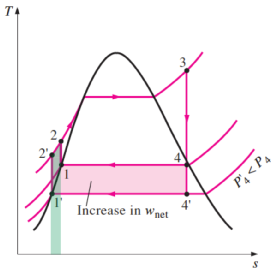
\includegraphics[scale=0.35]{ch9/image6.png}
		\captionof{figure}{ }
		\end{wrapfigure}
		On peut diminuer la pression dans le condensateur, cela augmente le 
		travail net (rose, $1'-2'-2-1-4'-4$), la chaleur fourmie au liquide 
		augmente aussi (augmente de $2'-2'$, vert) et l'efficacité thermique 
		augmente aussi. Cependant, réduire la pression réduit le titre et le 
		risque d'érosion augmente.\\\\
		\\
		
		
		\begin{wrapfigure}[8]{r}{3.cm}
		\vspace{-15mm}
		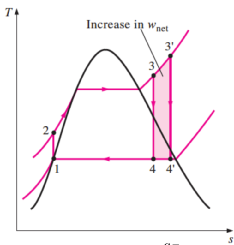
\includegraphics[scale=0.35]{ch9/image7.png}
		\captionof{figure}{ }
		\end{wrapfigure}
		Un autre moyen de faire est de surchauffer la vapeur. Le travail net 
		augmente (rose), la chaleur fournie au liquide aussi ($3-3'$), l'effet 
		net est une augmentation de l’efficacité et la teneur en eau en 4' 
		diminue. Hélas, l'irréversibilité augmente, la totalité du chauffage 
		est irréversible : le rendement exergétique diminue.\\\\
		
		
		\begin{wrapfigure}[7]{l}{3.cm}
		\vspace{-8mm}
		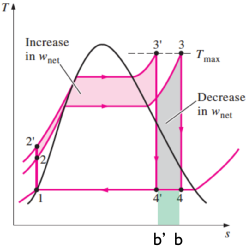
\includegraphics[scale=0.35]{ch9/image8.png}
		\captionof{figure}{ }
		\end{wrapfigure}		
		Troisième amélioration possible : augmenter la pression maximale. Le 
		travail net augmente (rose) et diminue en même temps (gris) : $w_{net}$ 
		est constant. Par contre, la chaleur rejetée par l'air diminue $4'-4-b
		-b'-4'$ et le rendement exergétique augmente. L'inconvénient est que la 
		teneur en eau augmente.\\
		\\
		
		\subsubsection{Alternative : cycle à resurchauffe}
		On introduit une ou plusieurs surfchauffe : l'efficacité est presque 
		constante, mais la teneaur en eau est réduit. L'idée est de faire une 
		détente incomplète puis de la re-réchauffer et effectuer une deuxième 
		détente, cette fois-ci complète. Ca fonctionne, mais il faut deux 
		turbines!
		\begin{center}
				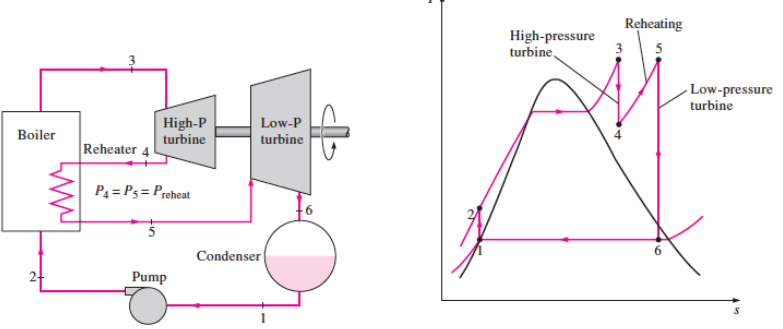
\includegraphics[scale=0.45]{ch9/image9.png}
		\captionof{figure}{Cycle à resurchauffe}
		\end{center}
	
		\subsubsection{Alternative : cycle a soutirage}
		La basse température est un problème niveau exergétique (on perd la plus 
		part de notre exergie). Ici, l'idée est de prélever une fraction de vapeur 
		dans la turbine à une pression intermédiaire pour réchauffer l'eau à la sortie 
		de la pompe. C'est mieux, car rajouter une turbine est plus compliqué 
		que de rajouter une pompe.
				\begin{center}
				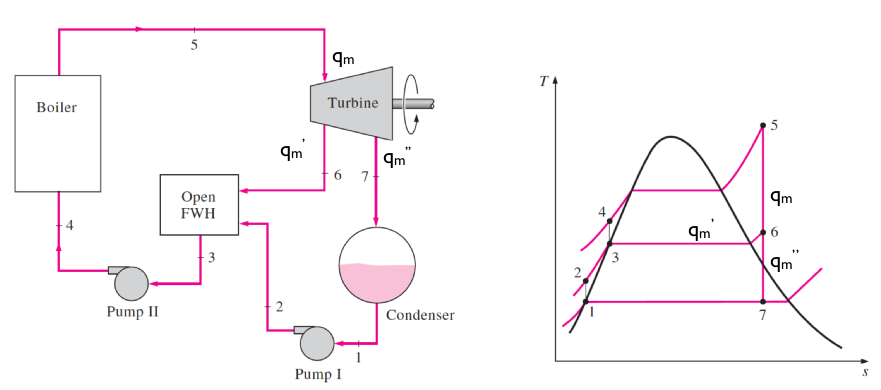
\includegraphics[scale=0.4]{ch9/image10.png}
		\captionof{figure}{Cycle à soutirage}
		\end{center}
		En pratique, plusieurs soutirages et des réchauffeurs d’eau à mélange
		sont utilisés. \textit{Le calcul du rendement est simple, mais pas intéressant.}
		
		
\newpage
\section{Cycles à gaz}
	
	
	
	
	
	
	
	
	
	
	
	
	
	
	
	
	
	